\chapter{Beyond This Book: Gaps and Projects}
\label{app:projects}

This book teaches the theory the assessment tests. It is meant to be studied together with three companion books: \emph{Book 1: HDLBits from Zero}, \emph{Book 2: After HDLBits, Step by Step}, and \emph{Book 3: Digital Hardware Foundations to Interview Practice}. This appendix says what the four books cover together, what none of them covers yet, and which projects turn that knowledge into an application that stands out.

\section{What the four books cover together}

\begin{center}
\small
\begin{tabularx}{\linewidth}{>{\raggedright\arraybackslash}p{4.4cm}>{\raggedright\arraybackslash}X}
\toprule
Book & What it gives you \\
\midrule
\emph{Hardware from the Ground Up} (this book) & The theory behind the multiple-choice section: electricity, transistors, CMOS gates, timing, power, PVT, wires, manufacturing rules, memory circuits, verification basics, architecture, GPUs, computer arithmetic, C traps, and a practice assessment. \\
\emph{Book 1: HDLBits from Zero} & Writing Verilog for the first time: widths, gates, multiplexers, K-maps, adders, registers, counters, state machines and simple testbenches, alongside the HDLBits exercises. \\
\emph{Book 2: After HDLBits, Step by Step} & Building and testing small systems in SystemVerilog: an ALU with flags, a timer, a FIFO, a UART transmitter, valid/ready pipelines, basic setup/hold, synchronizers and the FPGA flow. \\
\emph{Book 3: Digital Hardware Foundations to Interview Practice} & Interview-level RTL and verification: cocotb, assertions and UVM, timing constraints, asynchronous FIFOs, arbitration, caches, AXI and serial protocols, and interview drills. \\
\bottomrule
\end{tabularx}
\end{center}

Every topic candidates have reported for the Ignite hardware assessment is taught in at least one of the four. The overlap is small: this book explains \emph{why} circuits behave as they do, and the companions train you to \emph{build and verify} digital designs. Reading all four is not the same as mastering them, though, and a few things are still missing.

\section{What is still missing}
\label{sec:gaps}

\begin{enumerate}
  \item \textbf{Practice under time pressure.} Together the books contain only about fifty assessment-style questions plus chapter exercises, and one reported coding problem was harder than ``easy.''\\
  \emph{Close it:} redo every chapter's exercises under a timer, turn the formula sheet (Appendix~\ref{app:formulas}) into flash cards, and solve about three coding problems a week at LeetCode medium level in C or C++, focusing on linked lists, bit manipulation, hash maps and heaps.

  \item \textbf{Computer arithmetic in depth.} The Ignite posting lists it by name. Chapter~\ref{ch:arith} covers the core: overflow and saturation, fast adders, carry-save adders, multipliers and Booth recoding, division, fixed point, and floating-point addition, multiplication and rounding. What it does not cover is building and verifying these units at full width.\\
  \emph{Close it:} build Project~2's BF16 processing element and verify it against a reference model on millions of random and corner-case inputs. For more depth, read Parhami's \emph{Computer Arithmetic: Algorithms and Hardware Designs} or Koren's \emph{Computer Arithmetic Algorithms} (non-restoring and SRT division, prefix-adder families, rounding hardware).

  \item \textbf{Hands-on CUDA.} Chapter~\ref{ch:gpu} explains GPUs conceptually; the posting lists CUDA or OpenCL as a way to stand out.\\
  \emph{Close it:} work through NVIDIA's \emph{CUDA C++ Programming Guide} while doing Project~4.

  \item \textbf{Circuit simulation.} All of this book's transistor material is theory. Simulating the circuits yourself is what makes it stick.\\
  \emph{Close it:} Project~5.

  \item \textbf{The physical design flow.} Chapter~\ref{ch:fab} describes synthesis, placement, routing, timing sign-off, DRC, LVS and antenna checks, but you have not run them. Book 3 itself says physical design needs separate study.\\
  \emph{Close it:} Project~3.

  \item \textbf{CAD and MATLAB.} The posting lists mechanical CAD (Catia, Siemens NX, SolidWorks or Creo) and MATLAB. None of the books teach them, and they matter mainly for the power, thermal and mechanical teams.\\
  \emph{Close it:} only if those teams interest you; see Project~7.

  \item \textbf{Book 3's capstone targets a different industry.} Its capstone is an Ethernet/UDP market-data parser, aimed at FPGA and networking roles.\\
  \emph{Close it:} learn its methods, but build Projects~1 and~2 as your capstones instead.

  \item \textbf{Untested code.} Books 1--3 state that their HDL listings were reviewed but not run in a simulator.\\
  \emph{Close it:} type in and simulate every listing yourself. Fixing any that fail is excellent practice.
\end{enumerate}

\section{Check your eligibility}

Ignite accepts only first- and second-year undergraduates. In the 2027 cycle that meant the classes of 2030 and 2029, and the application window ran from October 5 to October 18, 2026. If you are a first-year now, you can apply to Ignite again next fall. If you are a second-year, next fall you will be a junior and should apply to NVIDIA's regular hardware internships instead. Those postings ask for more: the 2027 ASIC design and verification internships list RTL design, simulation, synthesis, static timing analysis, lint, CDC, and SystemVerilog with UVM or SVA. That makes the projects below even more important.

\section{What the job description asks for}

The 2027 Ignite Hardware Engineering posting requires coursework in hardware basics, basic knowledge of C, C++, Python, Perl or MATLAB, and involvement in clubs, leadership or extracurricular projects. Its ``ways to stand out'' list, and the teams interns can join, map onto the projects like this:

\begin{center}
\small
\begin{tabularx}{\linewidth}{>{\raggedright\arraybackslash}p{6.2cm}>{\raggedright\arraybackslash}X}
\toprule
What the posting asks for & Projects that show it \\
\midrule
Computer architecture & 1 (and 8) \\
Computer arithmetic & 2, 3 \\
VLSI design and CMOS circuits & 5, 3 \\
Verilog, SystemVerilog or VHDL & 1, 2, 3 \\
GPU APIs (CUDA or OpenCL) & 4 \\
Self-directed learning in AI and parallel computing & 2, 4 \\
CAD (Catia, Siemens NX, SolidWorks, Creo) & 7 \\
Programming in C, C++, Python, Perl or MATLAB & all (testbenches, scripts, analysis) \\
\midrule
\emph{Team:} GPU Verification and Design; Hardware ASIC & 1, 2 \\
\emph{Team:} ASIC Physical Design and Timing & 3, 5 \\
\emph{Team:} Hardware CPU Infrastructure & 1 \\
\emph{Team:} AI Developer Technology; HW Infrastructure Content/Performance & 4 \\
\emph{Team:} Power Architect & 6, 5 \\
\bottomrule
\end{tabularx}
\end{center}

\section{The plan: from transistor to software}

Five core projects together cover every layer of the hardware stack, which is exactly the story an NVIDIA interviewer wants to hear: you understand a design from the transistor up to the software that runs on it (Figure~\ref{fig:projectstack}).

\begin{figure}[h]
\centering
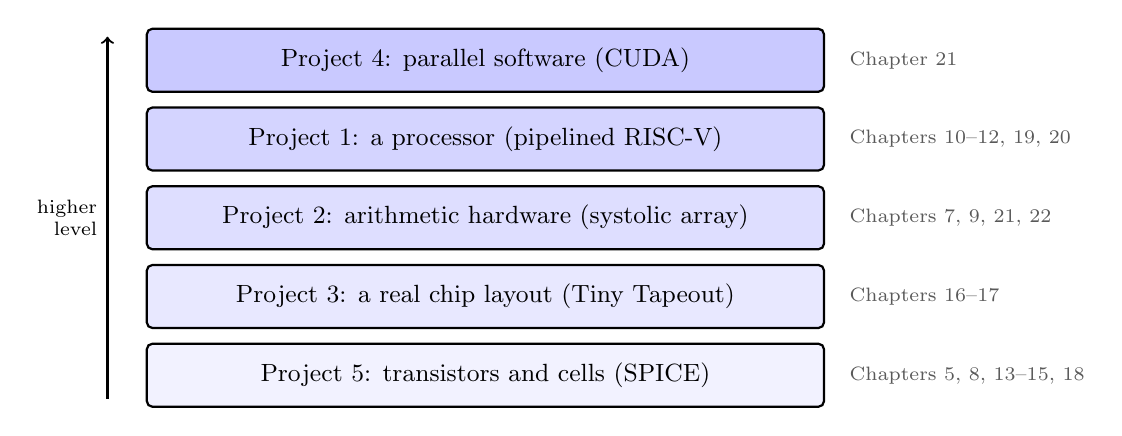
\begin{tikzpicture}[lvl/.style={draw,thick,rounded corners=2pt,minimum width=8.6cm,minimum height=0.8cm,font=\small}]
  \node[lvl,fill=blue!5]  at (0,0)   {Project 5: transistors and cells (SPICE)};
  \node[lvl,fill=blue!9]  at (0,1.0) {Project 3: a real chip layout (Tiny Tapeout)};
  \node[lvl,fill=blue!13] at (0,2.0) {Project 2: arithmetic hardware (systolic array)};
  \node[lvl,fill=blue!17] at (0,3.0) {Project 1: a processor (pipelined RISC-V)};
  \node[lvl,fill=blue!21] at (0,4.0) {Project 4: parallel software (CUDA)};
  \foreach \y/\t in {0/{Chapters 5, 8, 13--15, 18}, 1/{Chapters 16--17}, 2/{Chapters 7, 9, 21, 22}, 3/{Chapters 10--12, 19, 20}, 4/{Chapter 21}}
    \node[anchor=west,font=\scriptsize,gray!70!black] at (4.5,\y) {\t};
  \draw[->,thick] (-4.8,-0.3) -- node[left,font=\scriptsize,align=right]{higher\\level} (-4.8,4.3);
\end{tikzpicture}
\caption{The five core projects, from the lowest layer (transistors) to the highest (software), with the chapters each one exercises.}
\label{fig:projectstack}
\end{figure}

\begin{bigidea}
Three finished, verified, documented projects beat eight half-finished ones. The \textbf{minimum set} is Projects 1, 2 and 4, plus Project 3 whenever a Tiny Tapeout shuttle is open. Project 5 is small and directly strengthens your assessment knowledge, so do it early.
\end{bigidea}

All the tools below are free: Icarus Verilog or Verilator, cocotb, Yosys, nextpnr or the free edition of Vivado, OpenLane/OpenROAD, the SkyWater SKY130 process design kit, ngspice, Xschem, KiCad and the CUDA toolkit.

\section{Project 1: A pipelined RISC-V processor on an FPGA}

\textbf{Goal.} A processor you designed, verified, and ran a real program on.

\textbf{Build it in steps.}
\begin{enumerate}
  \item A single-cycle processor that executes the RV32I base instructions.
  \item Split it into the five stages of Chapter~\ref{ch:arch} (IF, ID, EX, MEM, WB). Add forwarding, the load-use stall and flushing on taken branches.
  \item Add a simple branch predictor (2-bit counters and a small branch target buffer) and measure how much it lowers CPI.
  \item Add a memory-mapped UART so a C program compiled with the RISC-V GCC toolchain can print text.
  \item Run it on an FPGA board. A low-cost Artix-7 board with the free Vivado edition, or a Lattice board with Yosys and nextpnr, both work.
\end{enumerate}

\textbf{Verify it.} Compare every retired instruction against a reference model (Spike, the official RISC-V simulator, or your own Python model) in a cocotb testbench. Run the official RISC-V architecture tests. Add SVA assertions for pipeline rules, and run random instruction sequences.

\textbf{Measure.} CPI on a small benchmark with and without branch prediction, maximum clock frequency from the timing report, and LUT, flip-flop and block-RAM usage.

\textbf{Shows:} computer architecture, SystemVerilog, verification. It also lets you answer ``what are the stages of a five-stage pipeline?'' with your own design. \textbf{Time:} about 10--12 weeks at 6--8 hours a week. \textbf{Stretch:} instruction and data caches, the M extension (hardware multiply and divide, which is computer arithmetic), interrupts.

\section{Project 2: A systolic-array matrix multiplier (a mini tensor core)}

\textbf{Goal.} Hardware for the operation that AI runs on, matrix multiplication (Chapter~\ref{ch:gpu}). This is the most NVIDIA-specific project in the plan.

A \term{systolic array} is a grid of small \term{processing elements} (PEs). Each PE multiplies the two numbers arriving from its neighbors, adds the product to a running sum, and passes the numbers on to the next PE in a steady rhythm, like a heartbeat (hence ``systolic''). Rows of one matrix flow in from the left and columns of the other flow in from the top (Figure~\ref{fig:systolic}). An $N \times N$ array performs $N^2$ multiply-adds every clock cycle.

\begin{figure}[h]
\centering
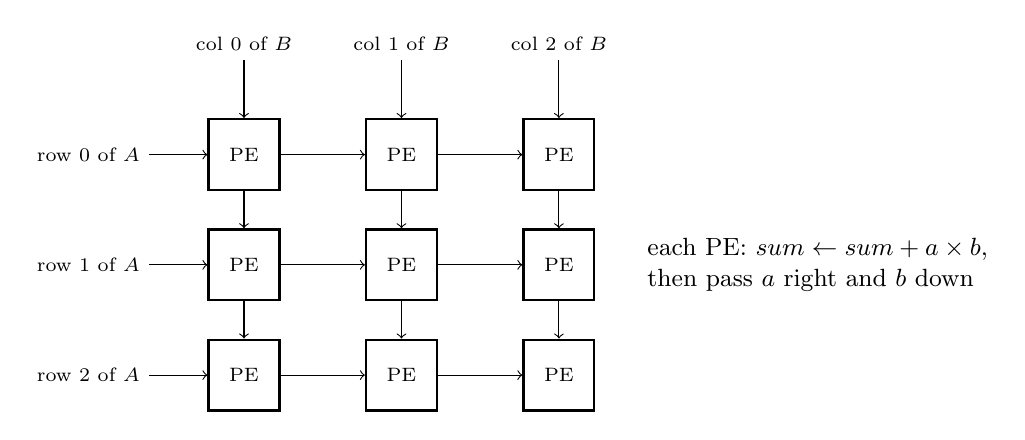
\begin{tikzpicture}[pe/.style={draw,thick,minimum size=0.9cm,font=\scriptsize}]
  \foreach \r in {0,1,2} \foreach \c in {0,1,2}
    \node[pe] (p\r\c) at (\c*2.0,-\r*1.4) {PE};
  \foreach \r in {0,1,2} {
    \draw[->] (-1.2,-\r*1.4) node[left,font=\scriptsize]{row \r\ of $A$} -- (p\r0.west);
    \draw[->] (p\r0.east) -- (p\r1.west); \draw[->] (p\r1.east) -- (p\r2.west);}
  \foreach \c in {0,1,2} {
    \draw[->] (\c*2.0,1.2) node[above,font=\scriptsize]{col \c\ of $B$} -- (p0\c.north);
    \draw[->] (p0\c.south) -- (p1\c.north); \draw[->] (p1\c.south) -- (p2\c.north);}
  \node[anchor=west,font=\small,align=left] at (5.0,-1.4) {each PE: $\text{sum} \leftarrow \text{sum} + a \times b$,\\then pass $a$ right and $b$ down};
\end{tikzpicture}
\caption{A $3 \times 3$ output-stationary systolic array. Each PE accumulates one element of the result matrix.}
\label{fig:systolic}
\end{figure}

\textbf{Build it in steps.}
\begin{enumerate}
  \item One PE: an INT8 $\times$ INT8 multiply feeding an INT32 accumulator.
  \item A $4 \times 4$ array with control for load, compute and drain.
  \item A host interface: a UART link from a PC, or memory-mapped registers on your Project~1 processor.
  \item A BF16 variant of the PE: multiply the significands, add the exponents, normalize, and round to nearest even. This is where computer arithmetic gets real.
\end{enumerate}

\textbf{Verify it.} In cocotb, compare the results bit for bit against NumPy for random matrices and corner cases such as $-128 \times -128$ and all-maximum inputs.

\textbf{Measure.} Multiply-adds per cycle, latency for an $N \times N$ product, maximum clock frequency and resources. Compare the achieved rate with the theoretical peak, PEs times clock frequency.

\textbf{Shows:} computer arithmetic, AI and parallel computing, VLSI, SystemVerilog. \textbf{Time:} about 6--8 weeks. \textbf{Stretch:} an $8 \times 8$ array, double buffering, INT4 or FP8 inputs.

\section{Project 3: Put a design on a real chip with Tiny Tapeout}

\textbf{Goal.} Take a design through the full physical design flow, and receive the manufactured chip.

\term{Tiny Tapeout} is an educational program that places many small designs side by side on one shared chip, so each person pays for only a small piece (a \term{tile}). It uses an open-source design flow and an open \term{process design kit} (PDK): the files that describe a factory's transistors and layout rules. Several shuttles (production runs) were offered during 2026. Dates and prices change, so check the Tiny Tapeout website for the next one.

\textbf{What to put on it.} Something small enough for a tile and its limited pins: a $2 \times 2$ version of Project~2, a Booth multiplier, or a compact state machine.

\textbf{Steps.}
\begin{enumerate}
  \item Write and verify the RTL with cocotb, using the program's project template.
  \item Run the automated flow to produce a layout (GDS file).
  \item Read every report: area, setup and hold slack, DRC and LVS results, and any antenna fixes. You can now explain the antenna rule (Section~\ref{sec:antenna}) from your own layout.
  \item Submit. When the chip arrives months later, test it and compare it with your simulation.
\end{enumerate}

\textbf{If no shuttle is open,} run OpenLane/OpenROAD on your own machine with the SKY130 PDK all the way to a layout. You will not get a chip, but you will have real physical design reports to discuss.

\textbf{Shows:} VLSI design, ASIC physical design and timing, CMOS. ``I taped out a chip'' is rare for a first- or second-year student. \textbf{Time:} about 4--6 weeks.

\section{Project 4: Optimizing matrix multiplication in CUDA}

\textbf{Goal.} Show that you can make a real NVIDIA GPU fast, and explain why each step helped, using Chapter~\ref{ch:gpu}.

\textbf{Steps.}
\begin{enumerate}
  \item A naive kernel: one thread computes one output element.
  \item Shared-memory tiling: each thread block loads tiles of the inputs once and reuses them.
  \item Register tiling: each thread computes a small block of outputs, reusing values held in registers.
  \item Vectorized loads, then (optionally) tensor cores through CUDA's WMMA interface with FP16 inputs.
  \item Compare each version with NVIDIA's cuBLAS library.
\end{enumerate}

\textbf{Measure.} GFLOP/s for each version at matrix sizes from 512 to 8192, as a percentage of cuBLAS. Profile with Nsight Compute (memory throughput, occupancy) and plot each version on a roofline chart. Then compare the GPU's multiply-adds per cycle with your Project~2 array.

\textbf{Hardware.} Any NVIDIA GPU: your own, a campus computing cluster, or a cloud notebook that offers one.

\textbf{Shows:} CUDA, parallel computing, AI. It fits the AI Developer Technology and performance teams especially well. \textbf{Time:} about 3--4 weeks.

\section{Project 5: Characterizing standard cells in SPICE}

\textbf{Goal.} See with your own simulations the transistor behavior this book describes. It is the fastest way to make the assessment's theory questions feel obvious.

Use ngspice and Xschem with the SKY130 PDK. Each experiment checks a chapter:
\begin{enumerate}
  \item An inverter's transfer curve, switching threshold and noise margins at several PMOS/NMOS size ratios (Chapter~\ref{ch:cmos}).
  \item An NMOS pass transistor's weak 1, and the swapped inverter from the assessment (Chapters~\ref{ch:mosfet} and~\ref{ch:cmos}).
  \item Delay versus fan-out, the FO4 delay, and a tapered buffer chain (Chapter~\ref{ch:delay}).
  \item Energy per transition versus supply voltage, to confirm the $CV^2$ law (Chapter~\ref{ch:power}).
  \item A temperature sweep from $-40$ to 125\,\textdegree C at normal and at low supply voltage, looking for temperature inversion (Chapter~\ref{ch:pvt}).
  \item A ring oscillator's frequency versus voltage and temperature.
  \item A 6T SRAM cell's read and write margins, and its butterfly curve (Chapter~\ref{ch:memory}).
\end{enumerate}

\textbf{Deliverable.} A short report with one plot per experiment, each compared with what this book predicts.

\textbf{Shows:} CMOS circuits, VLSI. \textbf{Time:} about 2--3 weeks.

\section{Track-specific options}

\paragraph{Project 6: GPU power and thermal characterization (power and infrastructure teams).} Log power draw, clock speed and temperature with \code{nvidia-smi} while running your Project~4 kernels at different sizes (and different clock settings, if your GPU allows it). Separate idle power from the extra power under load, fit the results to the $\alpha C V^2 f$-plus-leakage model of Chapter~\ref{ch:power}, estimate the energy per FLOP, and estimate the cooling system's thermal resistance from temperature rise versus power (Chapter~\ref{ch:heat}).

\paragraph{Project 7: Mechanical CAD (thermal and mechanical teams).} Design a heat sink, fan duct or enclosure in SolidWorks, Onshape or a similar tool. Size the fins and calculate the thermal resistance with Chapter~\ref{ch:heat}, then use the CAD tool's thermal simulation if it has one. Do the analysis in MATLAB or Python.

\paragraph{Project 8: A mini SIMT core (stretch goal).} Extend Project~1 into 4 to 8 lanes that execute one instruction stream on different data, with per-thread registers, an active mask for divergent branches, and a scheduler that switches between two warps. Run vector-add and matrix-add kernels and compare throughput with the scalar core. Open-source teaching designs such as tiny-gpu and the Vortex RISC-V GPGPU are worth studying for ideas, but write your own; interviewers will ask about every design decision.

\section{When to do what}

The month-by-month plan in Appendix~\ref{app:plan} fits the projects in alongside the reading. In short: Project~5 in January and March, Project~1 from February to April, Project~2 in May and June, Project~3 whenever a shuttle opens, Project~4 in July, and the track-specific projects in August if you want them.

\section{Making the projects count}

\paragraph{Each project's repository needs:}
\begin{itemize}
  \item[$\square$] a README with the specification, a block diagram and known limitations;
  \item[$\square$] one command that runs all the tests, ideally also run automatically on every push;
  \item[$\square$] a results table (clock frequency, resources, CPI, GFLOP/s or whatever the project measures);
  \item[$\square$] waveforms or plots that show the design working.
\end{itemize}

\paragraph{Writing resume bullets.} Each bullet says what you built, how you verified it, and a number you measured:

\begin{remember}
\begin{itemize}
  \item \textit{Designed a 5-stage pipelined RV32I processor in SystemVerilog with forwarding and branch prediction; verified against a reference model with cocotb, passing X of Y architecture tests; ran at Z\,MHz on an Artix-7 FPGA using N LUTs.}
  \item \textit{Built a 4$\times$4 INT8 systolic-array matrix multiplier, bit-exact against NumPy over X random tests; sustained Y multiply-adds per cycle at Z\,MHz.}
  \item \textit{Optimized CUDA matrix multiplication from X to Y GFLOP/s (Z\% of cuBLAS) with shared-memory and register tiling; analyzed each version with Nsight Compute and a roofline model.}
\end{itemize}
Replace X, Y, Z and N with numbers you actually measured. Never write a number you did not measure.
\end{remember}

\paragraph{The rest of the resume.} The posting requires your expected graduation month and year, and asks for clubs, leadership or extracurricular projects. A hardware-related club (IEEE, robotics, a solar-car or Formula team) or a hackathon project counts.

\paragraph{Be ready to defend every line.} Interviewers pick a project and dig: why these widths, what limits the clock frequency, what happens under backpressure, what the hardest bug was. Rehearse a two-minute explanation of each project, using Book 3's project deep-dive drill.
